%%%%%%%%%%%%%%%%%%%%%%%%%%%%%%
\subsection{Démarches critiques d'élicitation}

\subsubsection{Détecter et limiter les conflits entre prior et données }

Si rien formellement n'empêche de chercher à utiliser un prior $\theta\to \pi(\theta)$ et une vraisemblance qui, vue comme une fonction $\Theta\to\R^+$ ($\theta\to f(x_1,\ldots,x_n|\theta)$, peuvent être "éloignés" l'un de l'autre dans $\Theta$ (au sens où les régions de haute densité {\it a priori} favorisent d'autres zones que $\theta\to f(x_1,\ldots,x_n|\theta)$, ce type de situation doit être en pratique détecté. On parle de {\bf conflit entre prior et données} (même si ces deux objets ne vivent pas sur le même espace), qui peut aboutir à un calcul de posterior dont les régions HPD ne correspondent à aucune des zones privilégiées par les deux sources d'information. C'est donc un paradoxe qui a pour origine l'absence de règles d'élicitation du prior en cohérence avec la vraisemblance. \\

Afin de mieux appréhender ce problème, considérons l'exemple suivant. Soit un échantillon ${\bf x_n} \sim {\cal{N}}(\mu,\sigma^2)$. On suppose conna\^itre $\sigma$, mais $\mu$ est inconnu. On place l'{\it a priori} conjugué $\mu\sim{\cal{N}}(m,\rho\sigma^2)$. Peut-on émettre une règle simple de cohérence entre $\pi(\mu)$ et la vraisemblance des données ?   \\

On peut tenter de répondre à ce problème en utilisant des principes de statistique classique (fréquentiste), {\it via} une approche fondée sur la notion de {\it prior predictive check}.

\paragraph{{\bf Prior predictive check}.} En reprenant l'exemple précédent, on voit que $\bar{x}_n = \frac{1}{n}\sum_{i=1}^n x_i$ est une {\bf statistique exhaustive} de l'échantillon. Sous une hypothèse iid. des $X_i$, la loi de la variable aléatoire associée $\bar{X}_n$ est, conditionnellement à $(\mu,\sigma^2)$
\begin{eqnarray*}
\bar{X}_n|\mu,\sigma^2 & \sim & {\cal{N}}\left(\mu,\frac{\sigma^2}{n}\right).
\end{eqnarray*}   
 Intégrée sur $\pi(\mu)$, la loi {\it a priori prédictive} de $\bar{X}_n$ est
\begin{eqnarray*}
\bar{X}_n|\sigma^2 & \sim & {\cal{N}}\left(m,\sigma^2(\frac{1}{n} + \rho)\right).
\end{eqnarray*}
 Alors, {\it a priori} et {\it prédictivement a priori},
\begin{eqnarray*}
 Z_n & = & \frac{\left(\bar{X}_n - m\right)^2}{\sigma^2(\frac{1}{n} + \rho)}  \ \sim \ \chi^2_1.
\end{eqnarray*}
Il y a donc incohérence entre {\it a priori} et vraisemblance des données ${\bf x_n}$ si la valeur {\it observée} de  $Z_n$, à partir de $\bar{x}_n$, est une \emph{valeur extr\^eme} de la distribution du $\chi^2_1$. On cherche donc à "tester" le caractère extrême de la valeur observée de $Z_n$, ce qui revient à devoir définir de façon subjective (comme un niveau de $p-$value) une frontière. Ce choix peut avoir une forte influence, comme en témoignent les figures \ref{toto1} à \ref{toto5}. \\

Une autre problème subsiste : comment  justifier le choix d'une statistique "résumée", pour comparer sa valeur observée avec sa distribution {\it a priori} prédictive, plutôt qu'une autre ? Enfin, remarquons qu'il n'est pas évident que la loi sous $\theta$ de la statistique choisie (ici, $Z_n$) dépende complètement de toutes les dimensions de $\theta$. Dans le pire de cas, cette statistique peut être {\bf ancillaire/pivotale}, ce qui signifie qu'on ne peut l'utiliser pour détecter un conflit. Et hors de cas simples il n'est pas évident de vérifier qu'une statistique est bien ancillaire (ou pivotale). 

\begin{definition}{\bf Statistique pivotale ou ancillaire.}
Une statistique est appelée pivotale ou ancillaire par rapport au paramètre $\theta$ lorsque sa loi est indépendante de ce paramètre. 
\end{definition}

\clearpage

\begin{figure}[hbtp]
\centering
\begin{minipage}[b]{0.5\linewidth}
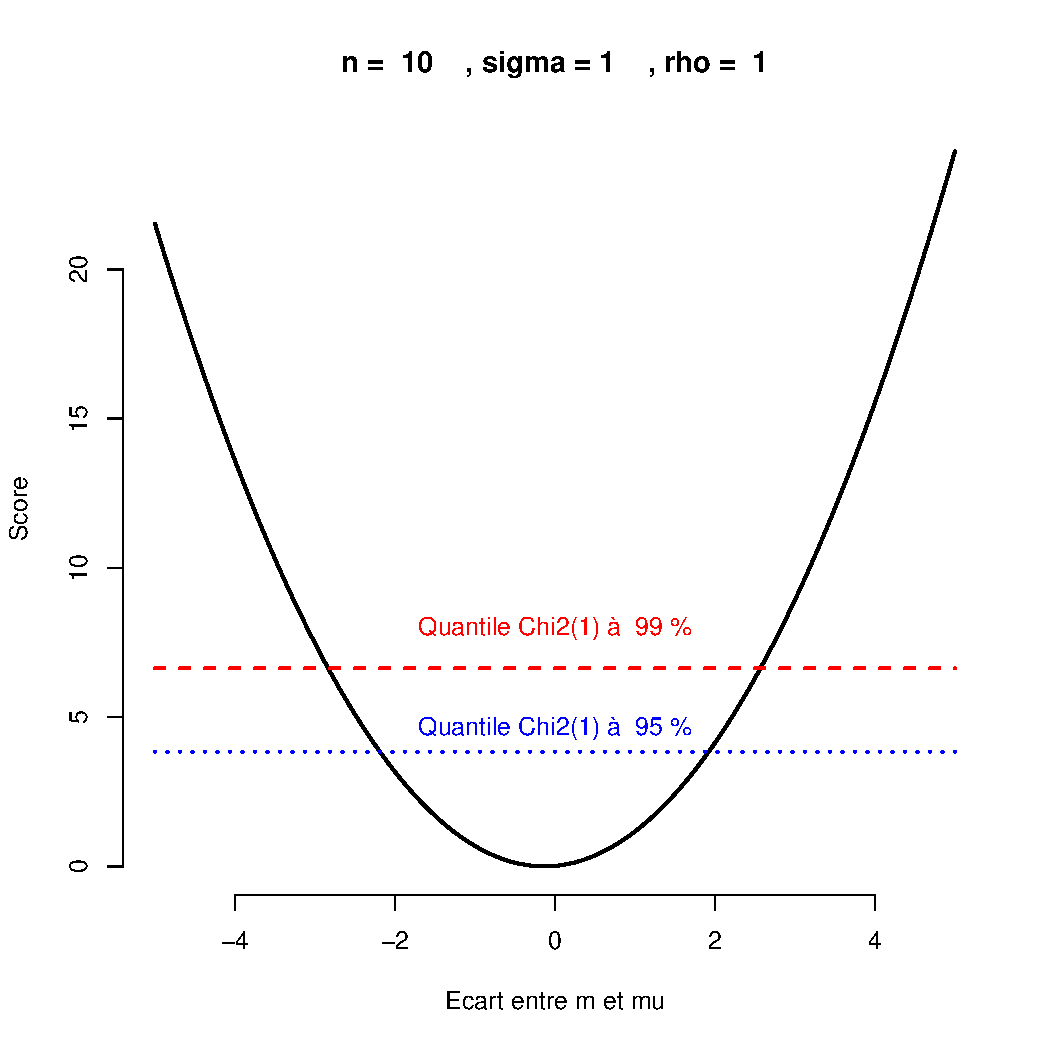
\includegraphics[scale=0.4]{figures/prior/figure1.pdf}
\caption{Influence du choix d'un seuil définissant le caractère extrême.}
\label{toto1}
\end{minipage}\hfill 
\begin{minipage}[b]{0.5\linewidth}
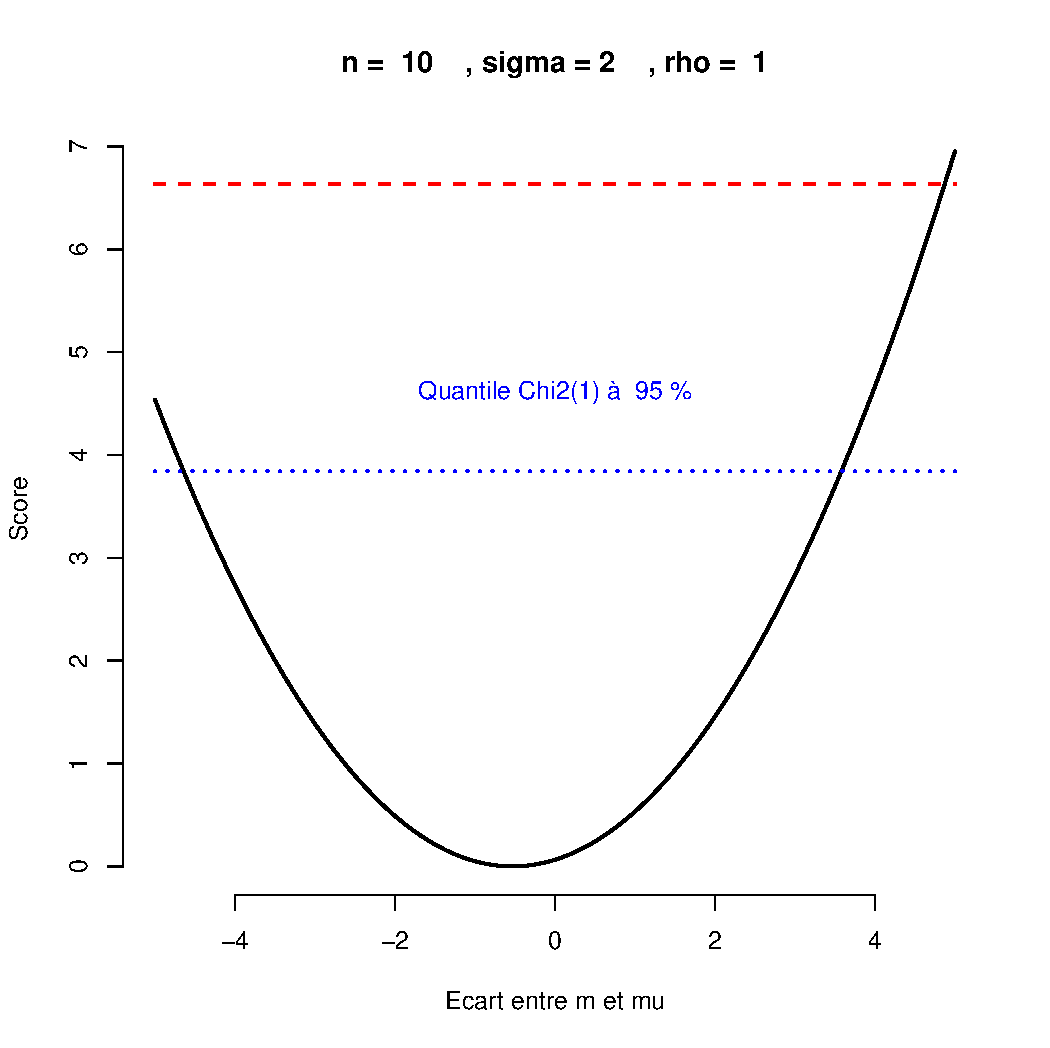
\includegraphics[scale=0.4]{figures/prior/figure2.pdf}
\caption{Influence d'un $\sigma$ plus large.}
\label{toto2}
\end{minipage}

\begin{minipage}[b]{0.5\linewidth}
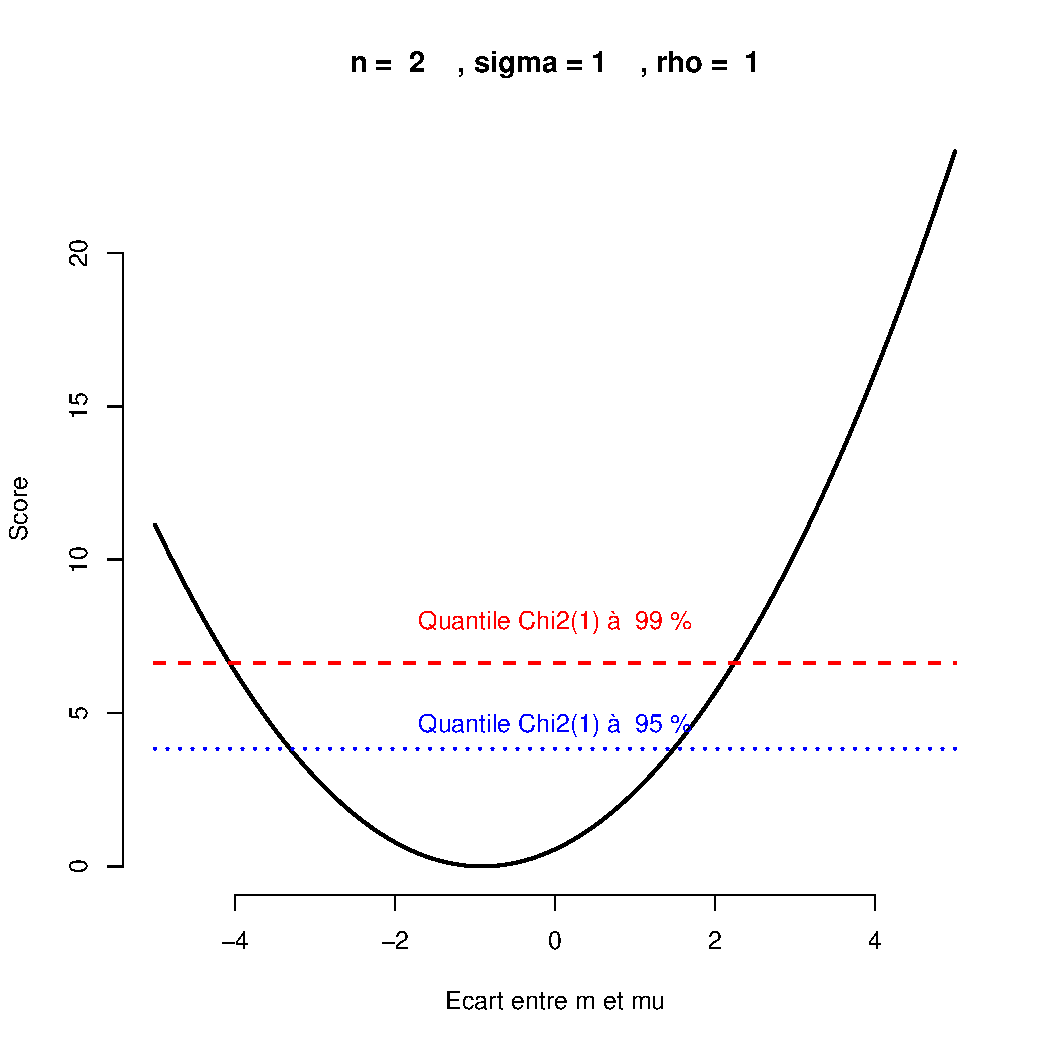
\includegraphics[scale=0.4]{figures/prior/figure3.pdf}
\caption{Influence d'une très faible taille d'échantillon.}
\label{toto3}
\end{minipage}\hfill 
\begin{minipage}[b]{0.5\linewidth}
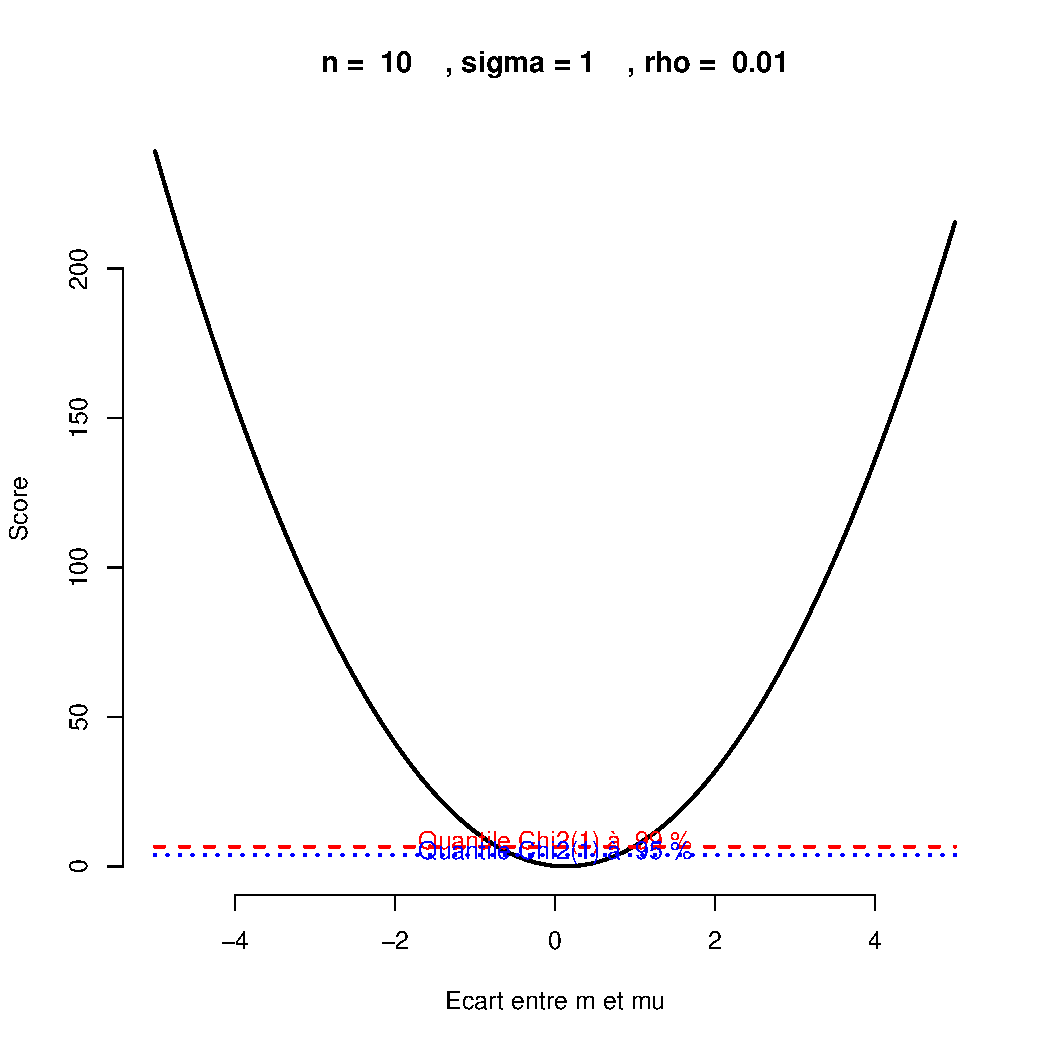
\includegraphics[scale=0.4]{figures/prior/figure4.pdf}
\caption{Influence d'une expertise extr\^emement précise.}
\label{toto4}
\end{minipage}

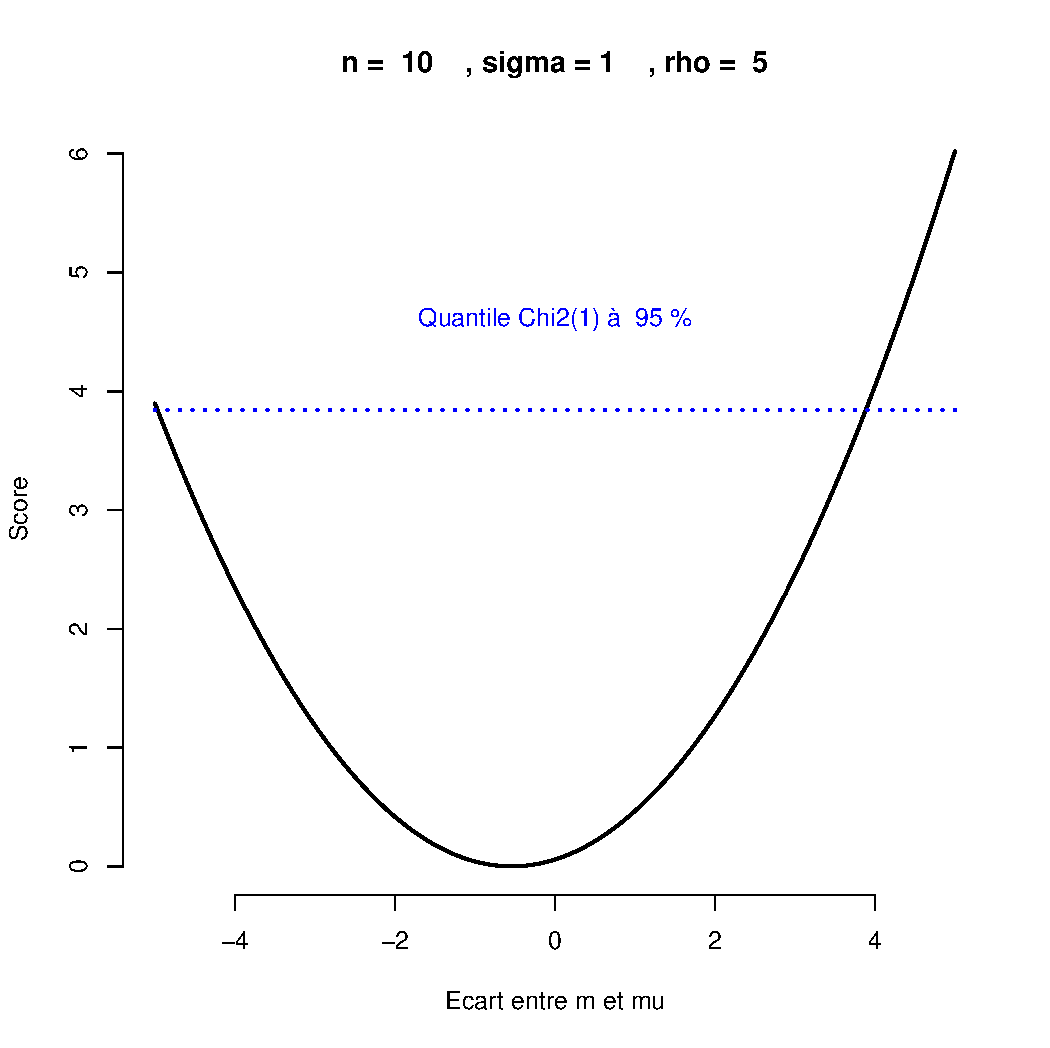
\includegraphics[scale=0.4]{figures/prior/figure5.pdf}
\caption{Influence d'une expertise extr\^emement vague.}
\label{toto5}

\end{figure}







\paragraph{{\bf Data-Agreement Criterion}.}
Pour remédier à la vision "fréquentiste" du problème de la détection de conflit, mais aussi pour évacuer le problème du choix de la statistique à tester, et enfin pour éviter le problème supplémentaire posé par les statistiques ancillaires, d'autres critères de détection ont été proposés. C'est le cas du critère DAC décrit ci-dessous. \\

Ce critère vise non pas à tester un désaccord entre sources d'information sur $X$ {\it via} un choix de statistique vivant dans l'espace des $X$, mais à tester un désaccord quand les sources d'information sont "projetées" dans l'espace $\Theta$. Il repose sur les hypothèses suivantes, dépendante d'un choix de prior "non informatif" pour l'expérience, noté $\pi^J$ :
\begin{enumerate}
    \item $\pi^J$ est toujours en accord avec les données ${\bf
 x_n}$ ;
    \item $\pi^J(\theta|{\bf x_n})$ est considéré comme une \emph{loi {\it a priori} 
"parfaite"}, correspondant à un expert fictif parfaitement en accord avec les données. 
\end{enumerate}
L'idée principale est que la divergence KL
\begin{eqnarray*}
D\left\{\pi^{J}(\theta|{\bf x_n}) \ || \ \pi(\theta)\right\}
\end{eqnarray*}
formule un regret informationnel dû au choix de states $\pi(\theta)$ alors que le choix de référence serait 
 $\pi^{J}(\theta|{\bf x_n})$. Quand $D\left\{\pi^{J}(\theta|{\bf x_n}) \ || \
\pi(\theta)\right\}$ est large, cela signifie un désaccord entre l'information {\it a priori} et l'information apportée par les données sur $\theta$. Supposons alors que $D\left\{\pi^{J}(\theta|{\bf x_n}) \ || \ \pi(\theta)\right\}>D\left\{\pi^{J}(\theta|{\bf x_n}) \ || \ \pi^J(\theta)\right\}$, et que $\pi(\theta)$ est plus informatif que $\pi^J(\theta)$. Nécessairement, le prior et les données sont en conflit. Cela permet de proposer le critère suivant.

\begin{definition}{\bf Data Agreement Criterion (DAC ; 2007).}
\begin{eqnarray*}
DAC^J(\pi|{\bf x_n}) & = &  \frac{D\left\{ \pi^{J}(\theta|{\bf
t_n}) \ || \ \pi(\theta)\right\}}{\ \ \ \ \ D\left\{
\pi^{J}(\theta|{\bf x_n}) \ || \
\pi^{J}(\theta)\right\}}.\label{coherstat}
\end{eqnarray*}
et $\pi$ et ${\bf
x_n}$ sont dits \emph{\it en conflit} si
$DAC^J(\pi|{\bf x_n})> 1$. 
\end{definition}

Une conséquence immédiate de cette définition est que lorsqu'on a affaire à un prior hiérarchique, on peut calculer DAC de fa\c con séparée à chaque niveau de la hiérarchie et obtenir le DAC pour le prior complet directement.  

\begin{proposition}{\bf Priors hiérarchiques.} 
Soit ${\pi(\theta)}  =
{\pi(\theta_1|\theta_2)\pi(\theta_2)}$ et
${\pi^J(\theta)}  =  {\pi^J(\theta_1|\theta_2)\pi^J(\theta_2)}$. \\
Soit 
$\textcolor{black}{\tilde{\pi}_1(\theta)}   = 
{\pi(\theta_1|\theta_2)}{\pi^J(\theta_2)}$ et 
$\textcolor{black}{\tilde{\pi}_2(\theta)} = 
{\pi^J(\theta_1|\theta_2)}{\pi(\theta_2)}$. \\
Alors
\begin{eqnarray*}
 \DAC({\pi}|{\bf x_n}) & = &
\DAC(\textcolor{black}{\tilde{\pi}_1}|{\bf x_n}) +
\DAC(\textcolor{black}{\tilde{\pi}_2}|{\bf x_n}) -1.
\end{eqnarray*}
\end{proposition}


\begin{proposition}{{\bf Fusion de priors} (voir $\S$ \ref{fusion}).}
Soit $$\pi(\theta)  \propto  \prod_{i=1}^M \pi_i(\theta)^{\omega_i}.$$ Alors
\begin{eqnarray*}
\DAC^J(\pi|{\bf x_n}) &  \leq & \sum\limits_{i=1}^M \omega_i \
DAC^J(\pi_i|{\bf x_n}). \ \ \ \text{(\emph{\scriptsize
arguments de convexité simples})}
\end{eqnarray*}
\end{proposition}


\begin{proposition}
Les priors réguliers ne sont pas en conflit avec ${\bf x_n}$ quand  $n\rightarrow \infty$:
\begin{eqnarray*}
\E\left[\DAC^J(\pi|{\bf x_n})\right] &\rightarrow & 1.
\end{eqnarray*}
\end{proposition}

\noindent Deux situations peuvent se présenter au statisticien :
\begin{enumerate}
\item\emph{\it Cas idéal}. $\Theta$ est borné et / ou 
${\cal{M}}(\theta)$ est discret. Alors $\pi^J$ est souvent  {\bf propre}:
\begin{eqnarray*}
\int_{\Theta} \pi^J(\theta) \ d\theta & < & \infty.\\
\end{eqnarray*}
\item\emph{\it Cas problématique}.  Si $\pi^J$ est impropre
 (ce qui arrive le plus souvent), le dénominateur de  DAC est défini à une 
\emph{\it
constante additive près inconnue}. Dans ce cas,  DAC ne peut pas être utilisé en l'état, et doit être adapté. \\
\end{enumerate}

\begin{exo}{Modèle gaussien borné.}\label{gauss100}
Supposons avoir \begin{eqnarray*}
{\bf x_n} & \overset{i.i.d.}{\sim} &
{\cal{N}}(\theta,1)\\
\theta & \sim & {\cal{N}}(\mu_0,\sigma_0) \ \ \text{restreint à 
$D=[-15,15]$}
\end{eqnarray*}
$\pi^J(\theta)$ étant la loi uniforme sur $D$. Dans ce cas, le calcul est aisé, et on peut par exemple tracer l'évolution de DAC en fonction de $\mu_0$ sur la figure \ref{postnormbounded1}. \\
\end{exo}

\begin{figure}[h!]
    \centering
    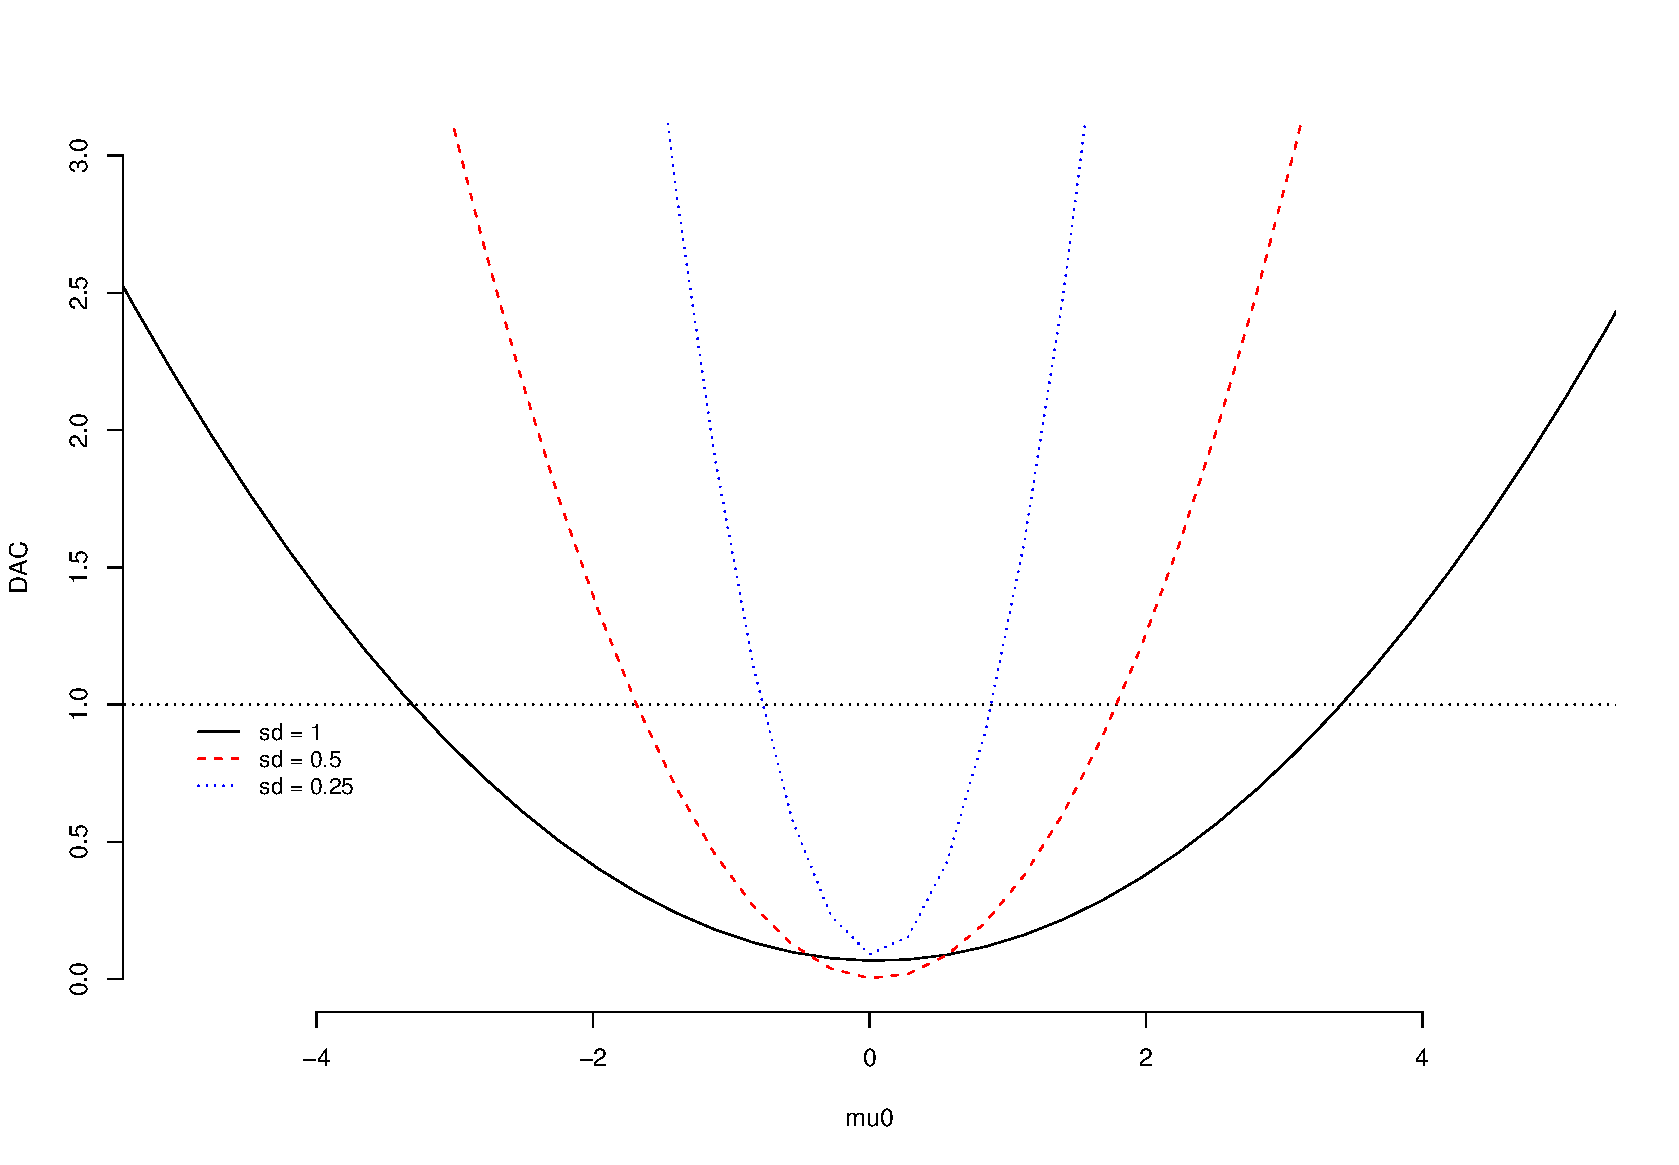
\includegraphics[scale=0.4]{figures/critics/postnormbounded1.pdf}
    \caption{Exemple \ref{gauss100}. Vraie valeur $\theta_0=0$, taille $n=5$}
    \label{postnormbounded1}
\end{figure}

Quand \emph{$\pi^J$ est impropre}, on a les mêmes difficultés conceptuelles que lorsqu'on souhaite calculer 
un 
\emph{facteur de Bayes}
\begin{eqnarray*}
 B_{J,\pi}({\bf
t_n}) & = & \frac{\int_{\Theta} {\cal{L}}({\bf x_n}|\theta)
\pi(\theta) \ d\theta}{\int_{\Theta} {\cal{L}}({\bf x_n}|\theta)
\pi^J(\theta) \ d\theta}\label{byf}
\end{eqnarray*}
qui est défini à une constante multiplicative inconnue près. En s'inspirant d'approches dites \emph{intrinsèques}, proposées originellement par Berger et Perrichi (1996, 1998), on peut proposer une adaptation en usant de \emph{petites quantités de données d'entraînement $x(l)\subset{\bf
t_n}$} pour remplacer \emph{le $\pi^J(\theta)$ impropre}
par un \emph{$\underbrace{\pi^J(\theta|x(l))}_{\text{\tiny "posterior prior"}}$ propre}. Le sous-échantillon $x(l)$ est appelé \emph{\it échantilllon minimal d'entraînement} (MTS). \\

\begin{definition}{\bf Critère DAC intrinsèque.}
Soit
${\bf x_n(-l)}={\bf x_n}/\{x(l)\}$ and $\ell$ la taille d'un MTS
$x(l)$. Par un argument de validation croisée
\begin{eqnarray*}
\DAC^{AIJ}(\pi|{\bf x_n}) & = & \frac{1}{L} \sum\limits_{l=1}^L
\frac{D\left\{\pi^J\left(.|{\bf x_n(-l)}\right) \ || \
\pi(.|x(l))\right\}}{ D\left\{\pi^J\left(.|{\bf x_n(-l)}\right) \
|| \ \pi^J\left(.|x(l)\right)\right\}}.\label{cohAIJ}
\end{eqnarray*}
\end{definition}

La qualité de l'adaptation est généralement bonne quand $L\geq 10$ et $n/\ell\geq 8$. Il reste cependant coûteux à calculer (sauf, évidemment, dans les cas conjugués). \\

\begin{exo}{Loi de Bernoulli.}\label{exo.bernoulli}
$X\sim {\cal{B}}_r(\theta)$ avec un prior de loi bêta. On choisit pour l'exemple $n=20$, une valeur de simulation 
$\theta_0=0.7$, et un prior $\theta \ \sim \ {\cal{B}}_e$ sur $[0,1]$, de moyenne
$\mu_0$ et pour un écart-type $\sigma=0.2$ fixé. Dans ce cas conjugué pour lequel le prior $\pi^J$ de Jeffreys est propre, on peut comparer les deux approches (figure \ref{betaglop1}). \\
\end{exo}


\begin{figure}[h!]
    \centering
    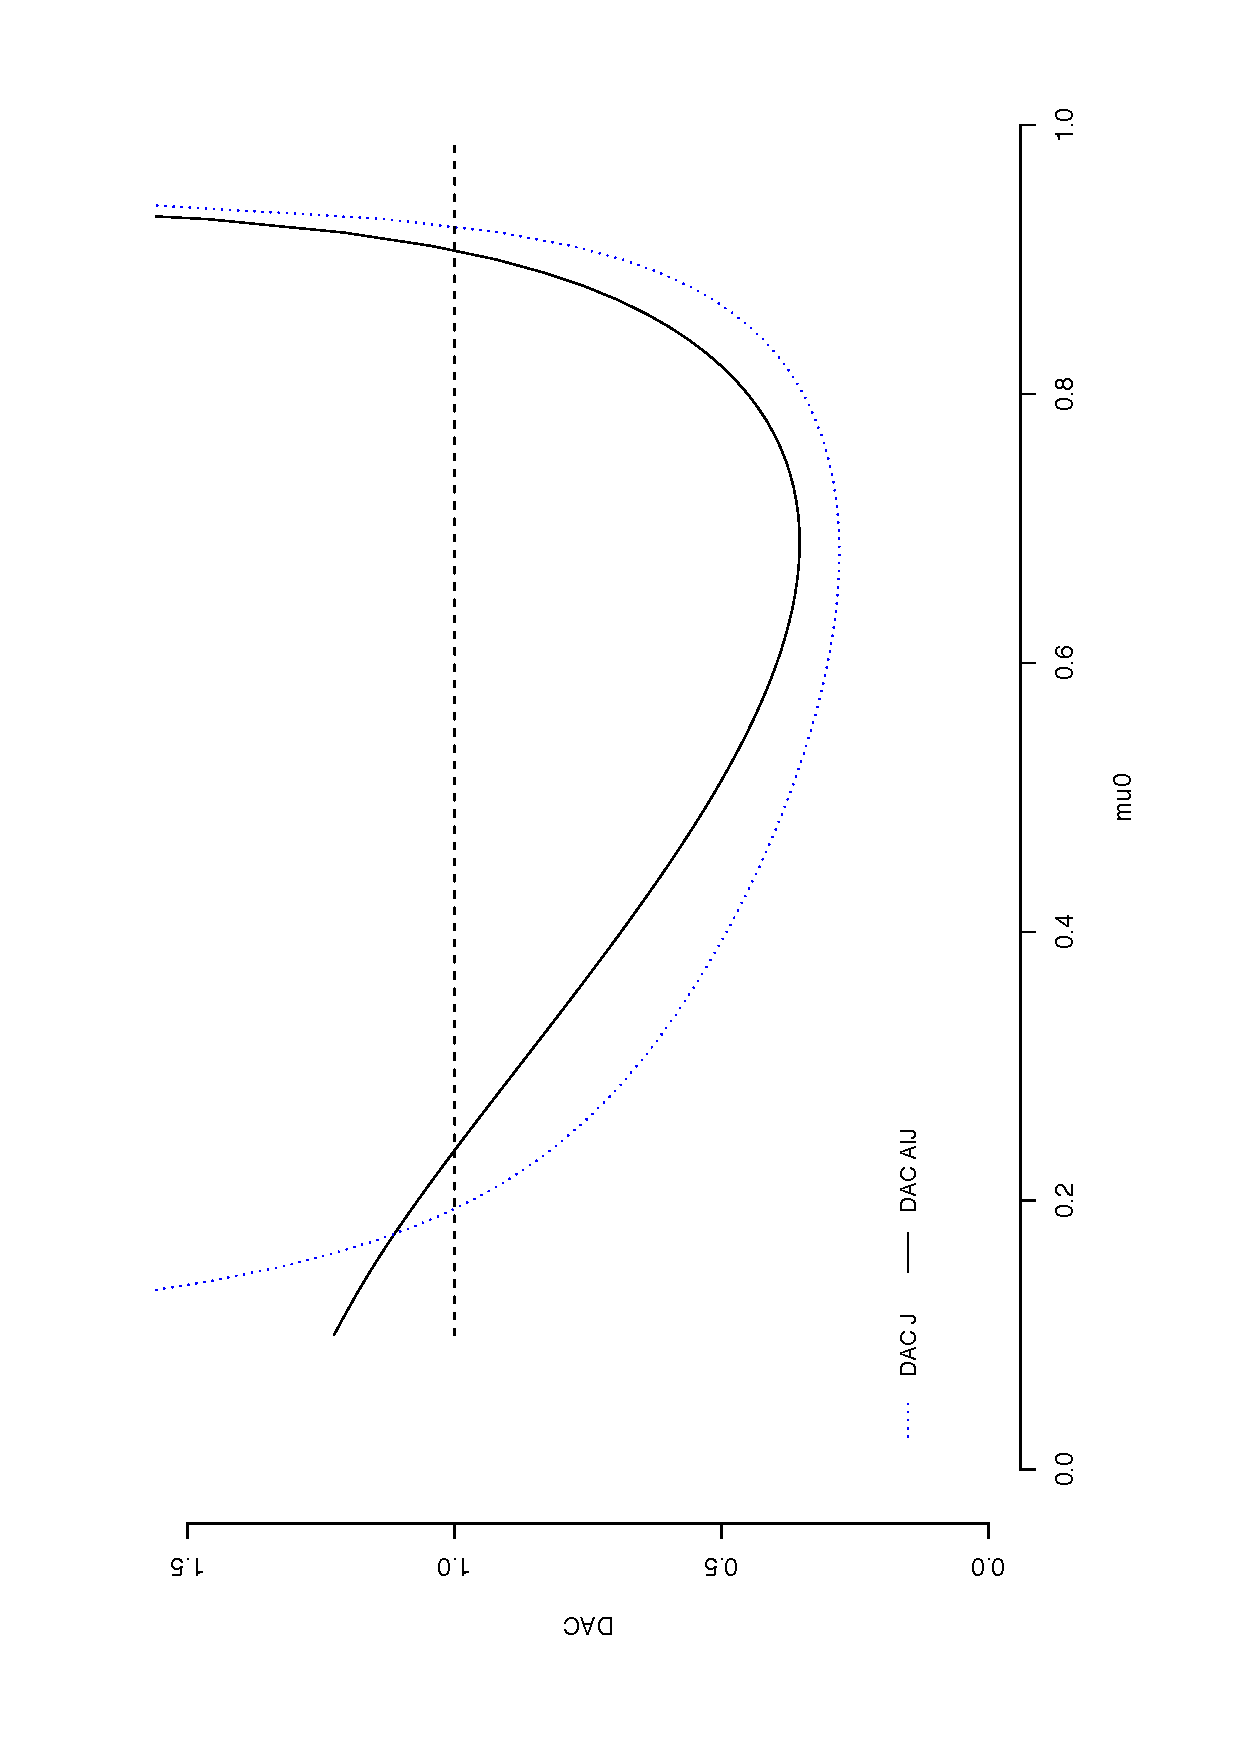
\includegraphics[scale=0.4,angle=270]{figures/critics/betaglop1.pdf}
    \caption{Exemple \ref{exo.bernoulli} : comparaison du DAC et du DAC intrinsèque.}
    \label{betaglop1}
\end{figure}


\begin{exo}{Loi exponentielle.}\label{exo.expo00}
Soit $X\sim {\cal{E}}(\lambda)$ avec $n=10$ et un EMV $\hat{\lambda}=207$. On choisit naturellement un prior conjugué $ \lambda  \sim  {\cal{G}}(a,a.te)$ et on décide de faire varier la "taille virtuelle $a$" et l'hyperparamètre $t_e$, qui correspond à la moyenne d'un échantillon virtuel (figure \ref{expograph}).  \\
\end{exo}

\begin{figure}[h!]
    \centering
    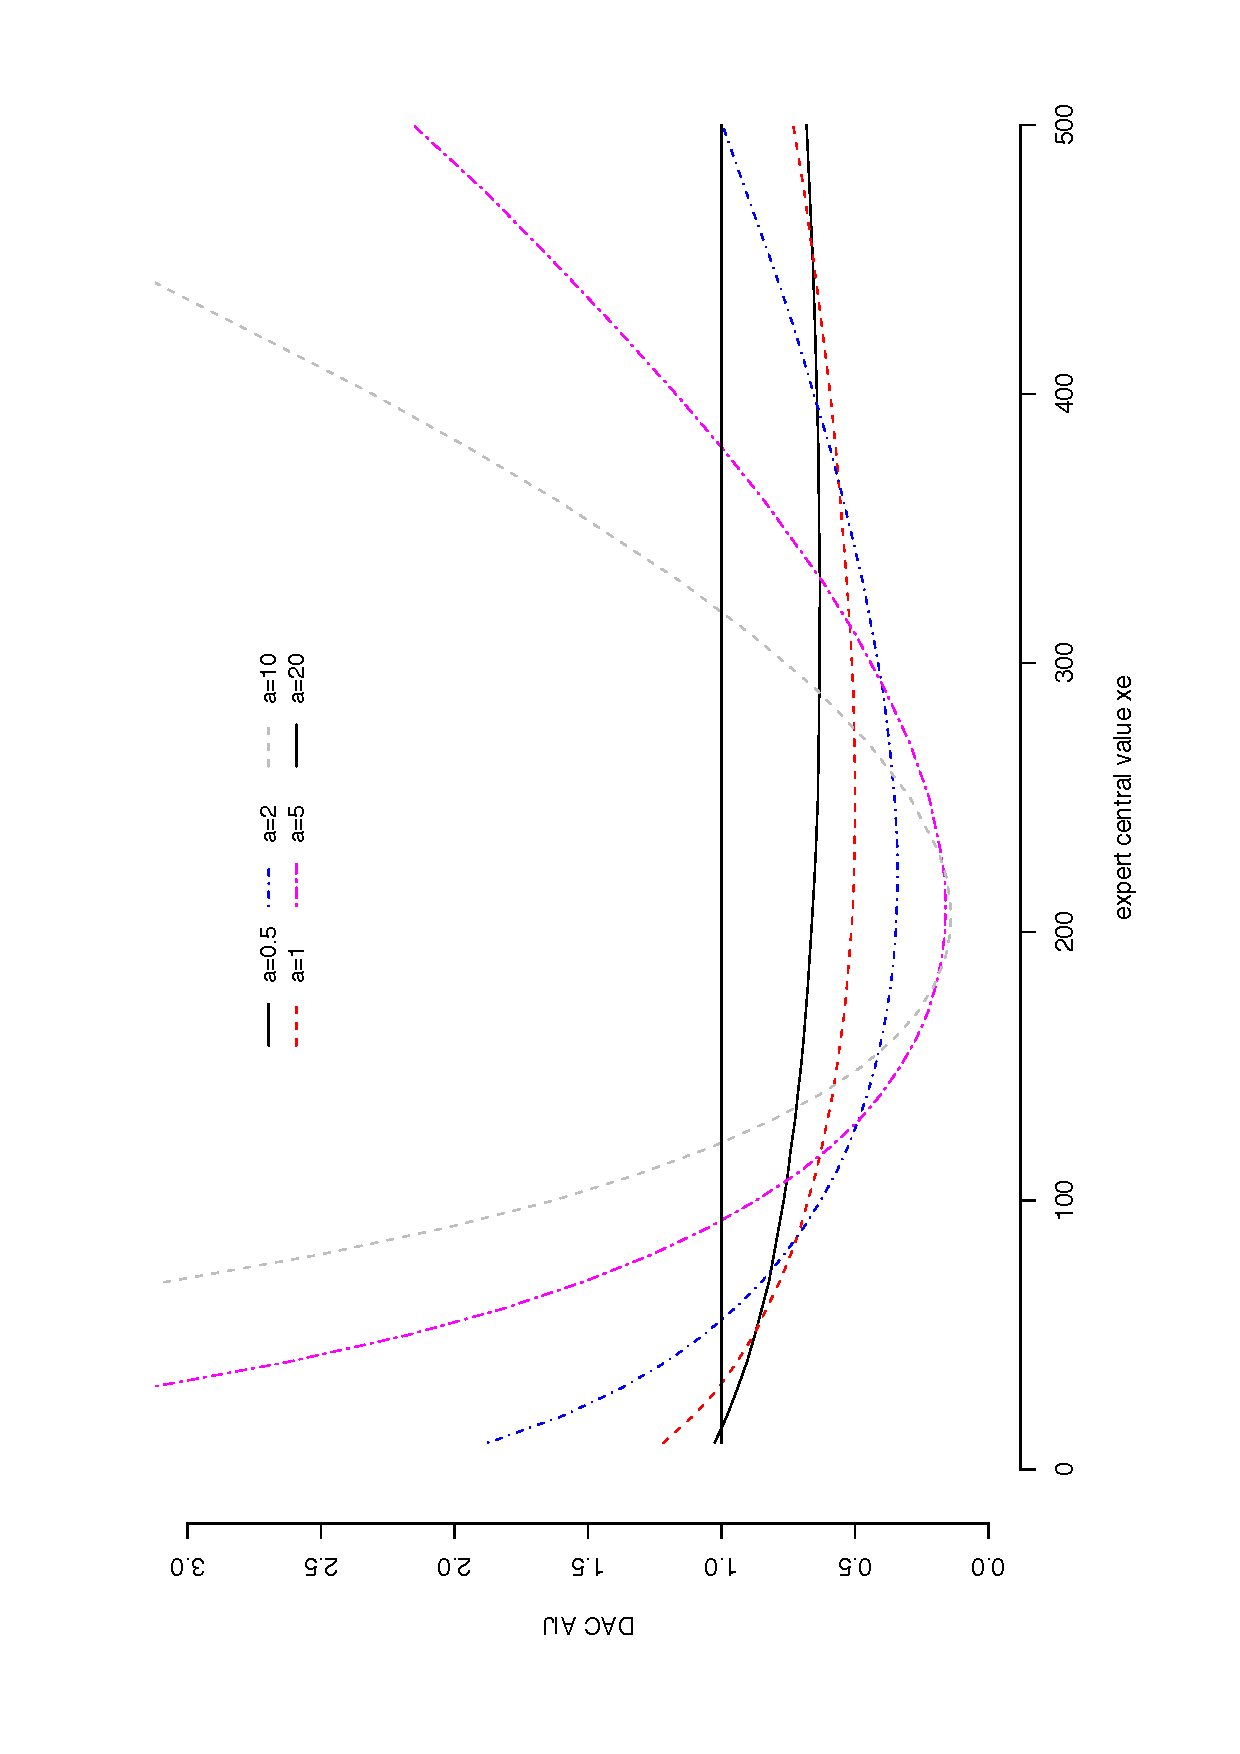
\includegraphics[scale=0.4,angle=270]{figures/critics/expograph1DACAIJ.pdf}
     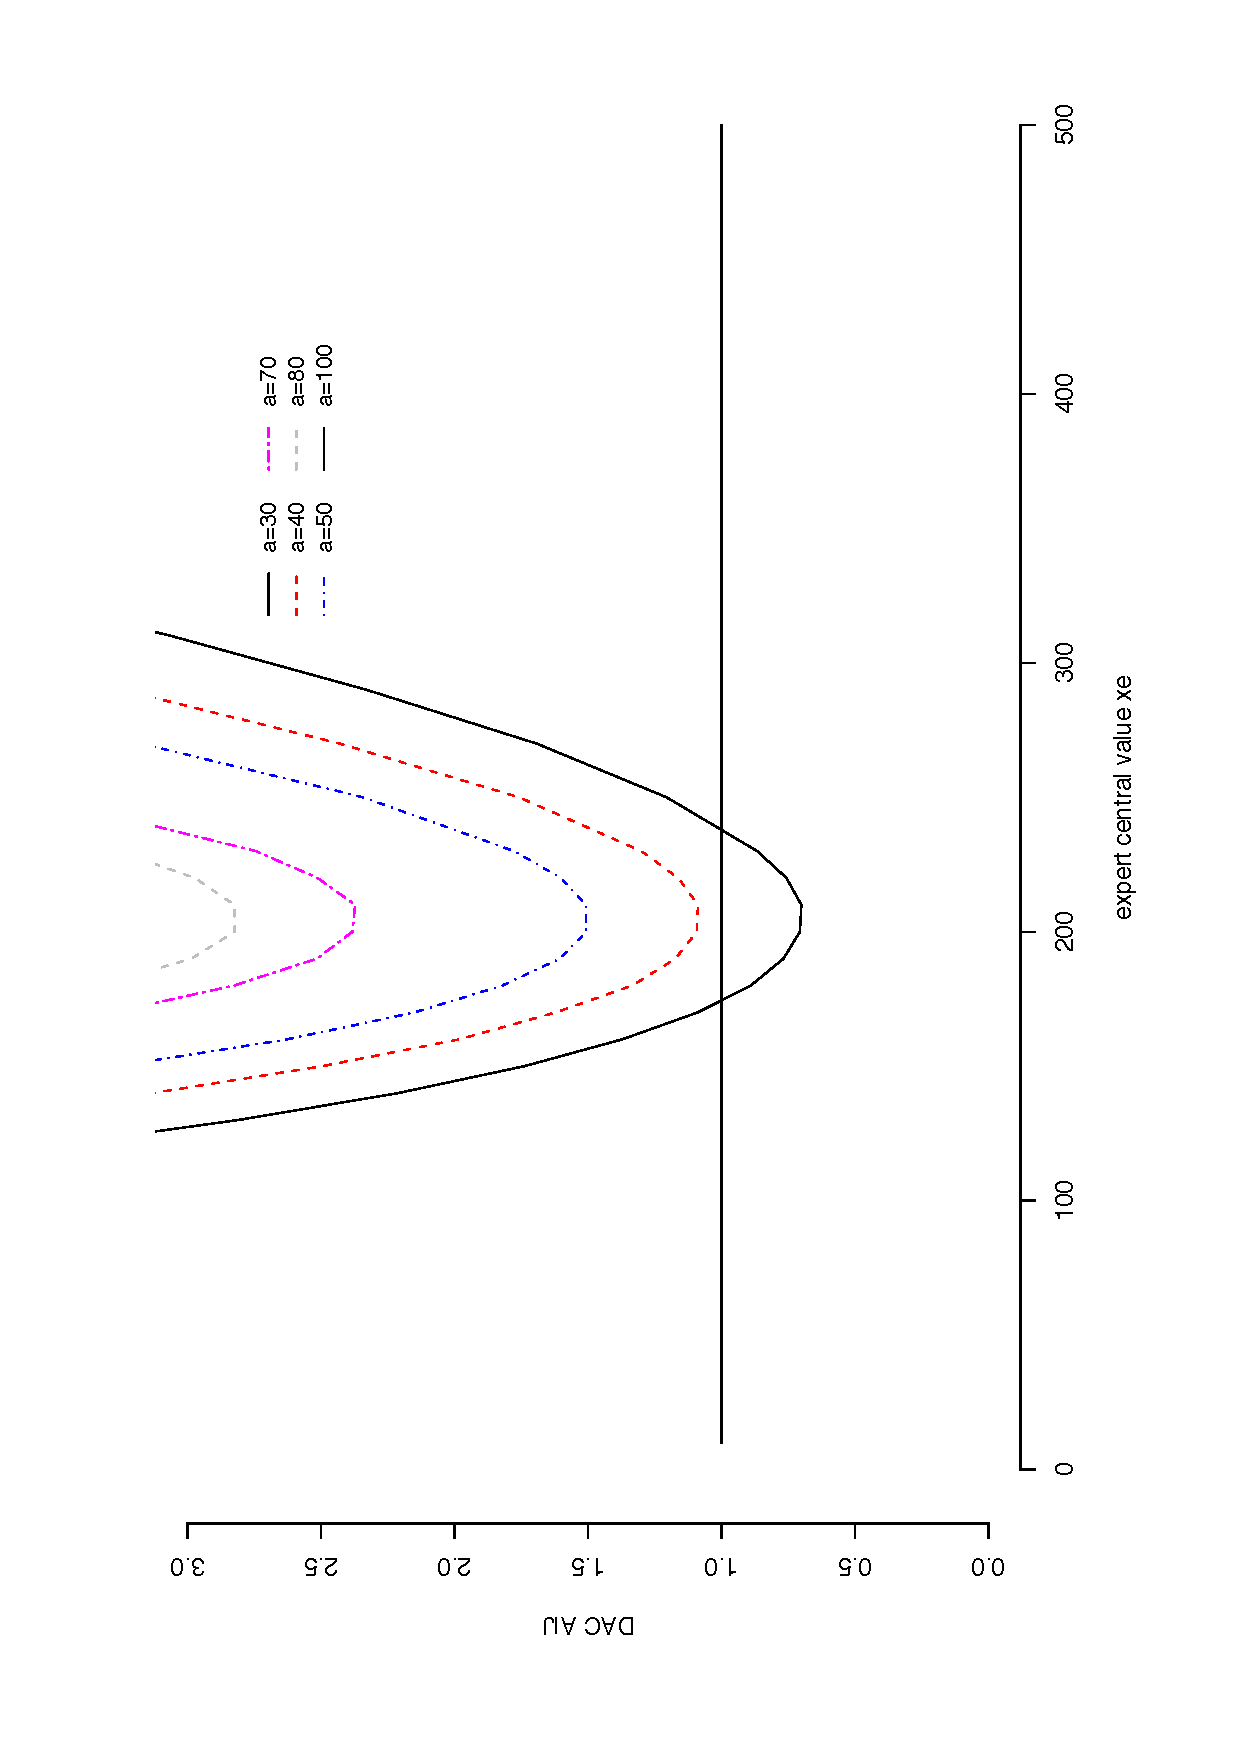
\includegraphics[scale=0.4,angle=270]{figures/critics/expograph2DACAIJ.pdf}
    \caption{Exemple \ref{exo.expo00} : DAC intrinsèques en fonction des variations des hyperparamètres.}
    \label{expograph}
\end{figure}


\noindent Le critère DAC présente en outre un avantage pour la calibration. En effet, $\DAC^J$ et $\DAC^{AIJ}$ détectent \emph{\it des priors très biaisés} et \emph{\it
des priors non biaisés mais trop informatifs} vis-à-vis des données ${\bf x_n}$. Si on se retrouve dans une situation où la seule information {\it a priori} dont nous disposons est une valeur centrale pour $\theta$, on peut souhaiter calibrer raisonnablement la taille virtuelle $m$ telle que
\begin{eqnarray*}
\DAC^{AIJ}(m^*|{\bf x_n})  &  = & 1.
\end{eqnarray*}

%%%%%%%%%%%%%%%%%%%%%%%%%%%%%%%%%%%%%%%%%%%%%%%%%%%%%%%%%%%%%%%%%%%%%%%%%%%%%%%
%\subsubsection{Priors compatibles pour la mise en concurrence des modèles}

%\emph{A CONTINUER}


%%%%%%%%%%%%%%%%%%%%%%%%%%%%%%%%%%%%%%%%%%%%%%%%%%%%%%%%%%%%%%%%%%%%%%%%%%%%%%%
\clearpage
\subsubsection{Fusionner plusieurs priors}\label{fusion}

Dans de nombreux cas pratiques, on peut disposer de plusieurs {\it a priori} possibles
$\pi_1(\theta),\ldots,\pi_M(\theta)$. \\ 

\begin{exo}
Réunions d'experts à la fin d'études pharmacologiques. \\
\end{exo}

Considérons d'abord la situation où les priors sont produits indépendamment les uns des autres. Une première idée est de proposer une {\bf fusion linéaire pondérée} (ou moyenne arithmétique) :
\begin{eqnarray*}
\pi(\theta) & = & \sum\limits_{i=1}^M \omega_i \pi_i(\theta)
\end{eqnarray*}
avec $\sum_{i=1}^M \omega_i=1$. Cette proposition n'est pas sans problème. En effet, le résultat produit peut être multi-modal, et contre-intuitif. De plus, cette approche n'est pas {\bf externalement bayésienne} :
\begin{eqnarray*}
\pi(\theta|{\bf x_n}) & \neq & \sum\limits_{i=1}^M \omega_i \pi_i(\theta|{\bf x_n})
\end{eqnarray*}
pour une ou plusieurs données ${\bf x_n}$. Cela pose un problème de cohérence. \\

Une autre approche est la {\bf fusion logarithmique pondérée} (ou moyenne géométrique) :
\begin{eqnarray*}
\pi(\theta) & = & \frac{\prod\limits_{i=1}^M  \pi^\omega_i(\theta)}{\int_{\Theta} \prod\limits_{i=1}^M  \pi^\omega_i(\theta) \ d\theta}
\end{eqnarray*}
avec $\sum_{i=1}^M \omega_i=1$. Celle-ci est bien externalement bayésienne. \\

Toutefois, elle pose un autre problème : elle n'est pas \emph{cohérente par marginalisation}. En fait, seule la fusion linéaire permet de respecter ce principe de cohérence. 

\begin{definition}{\bf Cohérence par marginalisation.}
Soit $A$ et $B$ tels que $A\cap B=\emptyset$ et $C=A\cup B$. Supposons avoir des systèmes experts indépendants produisant des estimateurs des probabilités des événements $A$ et $B$. Pour chacun, on peut directement calculer $P(C)$ ou calculer séparément $P(A)$ puis $P(B)$. La modélisation de ces experts est cohérente par marginalisation si  $P(C)=P(A)+P(B)$. 
\end{definition}

Mais la fusion logarithmique est globalement séduisante car elle peut s'expliquer en faisant appel à la théorie de l'information. Rappelons que la  divergence de Kullback-Leibler 
\begin{eqnarray*}
KL(\pi,\pi_i) & = & \int_{\Theta} \pi(\theta) \log \frac{\pi(\theta)}{\pi_i(\theta)}
\end{eqnarray*}
exprime une {perte en termes d'information} lorsque le meilleur choix {\it a priori} $\pi$ est remplacé par $\pi_i$. 

\begin{proposition}
Le minimiseur de la perte pondérée
\begin{eqnarray*}
\pi^*(\theta) & = & \arg\min\limits_{\pi} \sum\limits_{i=1}^M  \omega_i KL(\pi,\pi_i)
\end{eqnarray*}
est l'{\it a priori} opérant la fusion logarithmique. 
\end{proposition}


\if\mycmdproofthree1 \vspace{1cm} \begin{proof}% Log pooling
Soit $\{\pi_i\}_{i=1,\ldots,M}$ un ensemble de lois {\it a priori} sur $\Theta$. On pose
\begin{eqnarray*}
\pi^*(\theta) & = & \arg\min\limits_{\pi} \sum\limits_{i=1}^M \omega_i KL(\pi, \pi_i)
\end{eqnarray*}
avec $\sum_{i=1}^M \omega_i=1$ et $0\leq \omega_i \leq 1$ $\forall i=1,\ldots,M$. Alors, sous réserve que 
\begin{eqnarray*}
A & = & \int_{\Theta} \prod\limits_{i=1}^M \pi^{\omega_i}_i(\theta) \ d\theta \ < \ \infty,
\end{eqnarray*}
on a 
\begin{eqnarray*}
\pi^*(\theta) & = &  \arg\min\limits_{\pi} \sum\limits_{i=1}^M \omega_i \int_{\Theta} \pi(\theta) \log\frac{\pi(\theta)}{\pi_i(\theta)} \ d\theta, \\
& = &  \arg\min\limits_{\pi} \int_{\Theta} \pi(\theta) \left( \log \pi(\theta) - \log A^{-1}\prod\limits_{i=1}^M \pi^{\omega_i}_i(\theta) - A\right) \ d\theta, \\
 & = &  \arg\min\limits_{\pi} \left\{ KL\left(\pi || A^{-1}\prod\limits_{i=1}^M \pi^{\omega_i}_i(.)\right) - A\right\}, \\
 & = &  \arg\min\limits_{\pi}  KL\left(\pi || A^{-1}\prod\limits_{i=1}^M \pi^{\omega_i}_i(.)\right).
\end{eqnarray*}
et on en déduit que
\begin{eqnarray*}
\pi^*(\theta) & = & A^{-1}\prod\limits_{i=1}^M \pi^{\omega_i}_i(\theta). 
\end{eqnarray*}
\end{proof}
\fi
\vspace{0.5cm}

Notons cependant que la calibration des poids $\omega_i$ est un problème qui reste ouvert, malgré quelques réponses déjà proposées. Un dernier argument plaide pour ce choix de fusion. La famille exponentielle naturelle est stable par ce type de fusion, et cette fusion correspond naturellement à celle réalisée par une nférence bayésienne croissante, indépendante de l'ordre d'arrivée des informations (ex : échantillons virtuels).  \\

\noindent Il n'existe pas de démarche canonique pour traiter la situation où les priors sont produits dépendamment les uns des autres. Les approches par \emph{copules} peuvent être utilisées si l'on connaît explicitement la structure de dépendance. On peut aussi considérer que les (systèmes) experts produisant les priors $\pi_i$ sont des générateurs aléatoires dépendants de valeurs de $\theta$, et une démarche de construction hiérarchique {\it a priori} peut alors être proposée. 

\begin{exec}
Considérons $M$ priors exponentiels 
\begin{eqnarray*}
\theta & \sim & \pi_i(\theta) \ = \ \lambda_i \exp(-\lambda_i \theta) \1_{\{\theta\geq 0\}}.
\end{eqnarray*}
Quelle est la loi-fusion logarithmique ?
\end{exec}



%%%%%%%%%%%%%%%%%%%%%%%%%%%%%%

%%%%%%%%%%%%%%%%%%% TP avec correction %%%%%%%%%%%%%%%
\clearpage
 \subsection{TP : Un exemple complet dans un cadre de fiabilité industrielle }

Soit $X$ la durée de vie d'un composant $\Sigma$, supposé tomber uniquement en panne par hasard. Le taux de défaillance $\lambda$ de $\Sigma$ est donc constant, ce qui implique  $X\sim {\cal{E}}(\lambda)$. Il est courant de disposer d'un  expert industriel  familier de $\lambda$, avec qui le dialogue suivant peut être engagé. 
 "Considérons une décision de management (remplacement) établie sur une valeur donnée $\bar{\lambda}$ \emph{(différente de la vraie valeur inconnue $\lambda$)}
\item Pour un \emph{co\^ut} similaire  $|\bar{\lambda}-\lambda|$, il y a 2 conséquences possibles au remplacement : 
\begin{itemize}
\item  soit $C_1$ le co\^ut positif moyen d'\^etre trop optimiste (d'avoir $\bar{\lambda}\leq \lambda$) ; 
\item  soit $C_2$ le co\^ut positif moyen d'\^etre trop pessimiste (d'avoir $\bar{\lambda}>\lambda$). 
\item Pouvez-vous donner un estimé $\hat{\delta}$ du rapport des co\^uts moyens $\delta=C_2/C_1$" ?
\end{itemize}
L'axiome de rationalité dit que si l'expert n'est pas \emph{averse au risque}, alors 
\begin{eqnarray*}
\bar{\lambda} & = & \arg\min_{x} \underbrace{\int_{0}^{\infty} \left|x-\lambda\right|\left(C_1\1_{\{x\leq \lambda\}} + C_2\1_{\{x>\lambda\}}\right) \pi(\lambda) \ d\lambda}_{\text{\tiny fonction de co\^ut intégr\'ee sur toutes les valeurs possibles {\it a priori} du vrai $\lambda$}} 
\end{eqnarray*}
\begin{eqnarray*}
\text{ Il s'ensuit que} \ \ \ \ \int_{0}^{\bar{\lambda}} d\Pi(\lambda) & = & \Pi(\lambda<\bar{\lambda}) \ = \ \frac{C_1}{C_1+C_2}.  
\end{eqnarray*} 
 L'interprétation de la réponse de l'expert est que $1/(1+\hat{\delta})$ est un estimé du quantile {\it a priori} d'ordre $\alpha=C_1/(C_1+C_2)$. 
Avec $P(\lambda<\bar{\lambda})=\frac{C_1}{C_1+C_2}=\alpha$, on a :
\begin{itemize}
\item tant que les co\^uts sont équilibrés, un expert de plus en plus optimiste fournira un $\bar{\lambda}$ de plus en plus petit, car la durée moyenne avant la prochaine défaillance est
\begin{eqnarray*}
\E[X|\lambda] & = &  \frac{1}{\lambda}.
\end{eqnarray*}
 
\item cependant l'expert s'exprime plutôt sur les co\^uts lorsqu'on lui fournit une valeur représentative de $\bar{\lambda}$ : 
\begin{itemize} 
\item   plus l'expert est optimiste, plus le co\^ut $C_2$ d'\^etre optimiste (selon lui) est petit, donc $\alpha$ grandit vers 1 et
\begin{eqnarray*}
\E[X] & = & \E[\E[X|\lambda]] \ = \ \E[1/\lambda] \ \ \text{augmente}.
\end{eqnarray*}
\item   plus l'expert est pessimiste, plus le co\^ut $C_2$ d'\^etre optimiste augmente, donc $\alpha$ tombe vers 0 et
\begin{eqnarray*}
\E[X] & = &  \E[1/\lambda] \ \ \text{diminue}.
\end{eqnarray*}
\end{itemize}
\end{itemize} 
Quelle choix de loi {\it a priori} pouvons-nous proposer au décideur ?



\if\mycmdtpthree1 \paragraph{\bf Réponse.} \\

On raisonne par \emph{données virtuelles} : 
\begin{itemize}
\item L'{\it a priori} non-informatif de Jeffreys est utilisé pour modéliser l'absence d'expertise et la simple connaissance du modèle 
\begin{eqnarray*}
\pi_{0}(\lambda) & \propto \lambda^{-1}  \ \ \ \ \ \ \ \ \text{ {\it (paramètre d'échelle)}}. 
\end{eqnarray*} 
\item L'information apportée par l'expert est assimilée à celle apportée par un échantillon i.i.d. 
\begin{eqnarray*}
{\bf x_m} & \sim & {\cal{E}}(\lambda).
\end{eqnarray*}
\item Un ``bon" prior informatif pour $\lambda$ est donc $\pi(\lambda)=\pi_0(\lambda|{\bf x_m})$, soit
\begin{eqnarray*}
\lambda & \sim & {\cal{G}}(m,m \bar{\bf x}_m).
\end{eqnarray*} 
\end{itemize}
Donc $2m \bar{\bf x}_m \lambda \sim {\cal{G}}(m,1/2) \equiv \chi^2_{2m}$, d'où ${\displaystyle \bar{\bf x}_m  =  \frac{\chi^2_{2m}(\alpha)}{2m\bar{\lambda}}}$. Le décideur peut fixer arbitraitement $m$ selon la confiance qu'il a en l'expert {(ou mettre un {\it a priori} hiérarchique dessus)}. De plus, l'{\it a priori} est \emph{conjugué} : sachant des durées de vie observées ${\bf x_n}=(x_1,\ldots,x_n)$, la loi {\it a posteriori} de $\lambda$ est
\begin{eqnarray*}
\lambda|{\bf x_n} & \sim & {\cal{G}}\left(m+n,\frac{\chi^2_{2m}(\alpha)}{2\bar{\lambda}} + n\sum\limits_{i=1}^n x_i\right)
\end{eqnarray*} 
L'ingénieur s'intéresse alors à la probabilité \emph{prédictive} que $\Sigma$ tombe en panne avant la prochaine visite au temps $x_0$
\begin{eqnarray*}
P\left(X<x_0\right)  & = & \int_{0}^{\infty} P\left(X<x_0|\lambda\right) \pi(\lambda|{\bf x_n}) \ d\lambda \ = \ 
                   1 - 1/\left(1 + \frac{x_0}{\frac{\chi^2_{2m}(\alpha)}{2\bar{\lambda}} + n\sum\limits_{i=1}^n x_i}\right)^{m+n}
\end{eqnarray*}
puis il peut introduire une fonction de co\^ut, etc. pour prendre une décision. Les figures suivantes (\ref{expert1} à \ref{expert3}) illustrent ainsi différents comportements {\it a posteriori}, lorsqu'on simule 10 données selon ${\cal{E}}(\lambda_0)$ avec $\lambda_0=1/10$. \\ 

\begin{figure}[h!]
\centering
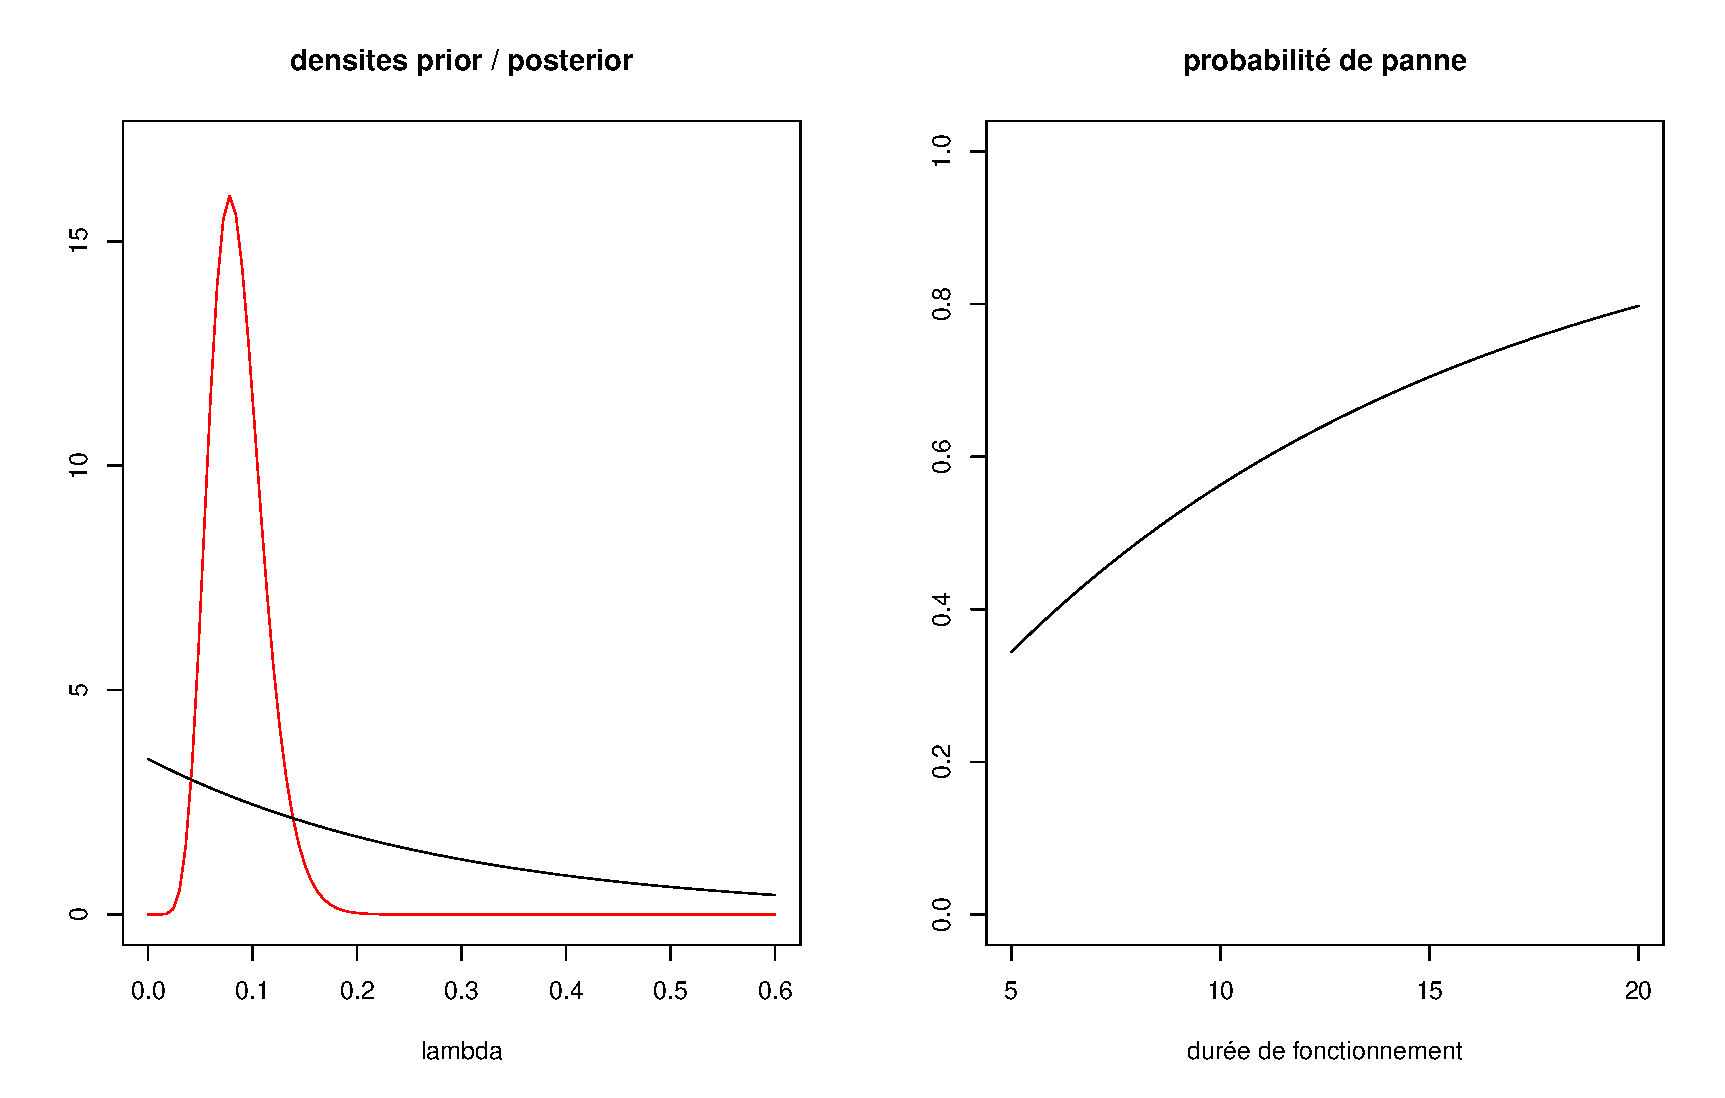
\includegraphics[scale=0.4]{figures/prior/figure01.pdf} 
\caption{$m=1$, $\bar{\lambda}=1/5$, $\alpha=50\%$ (expert peu informatif et pessimiste).}
\label{expert1}
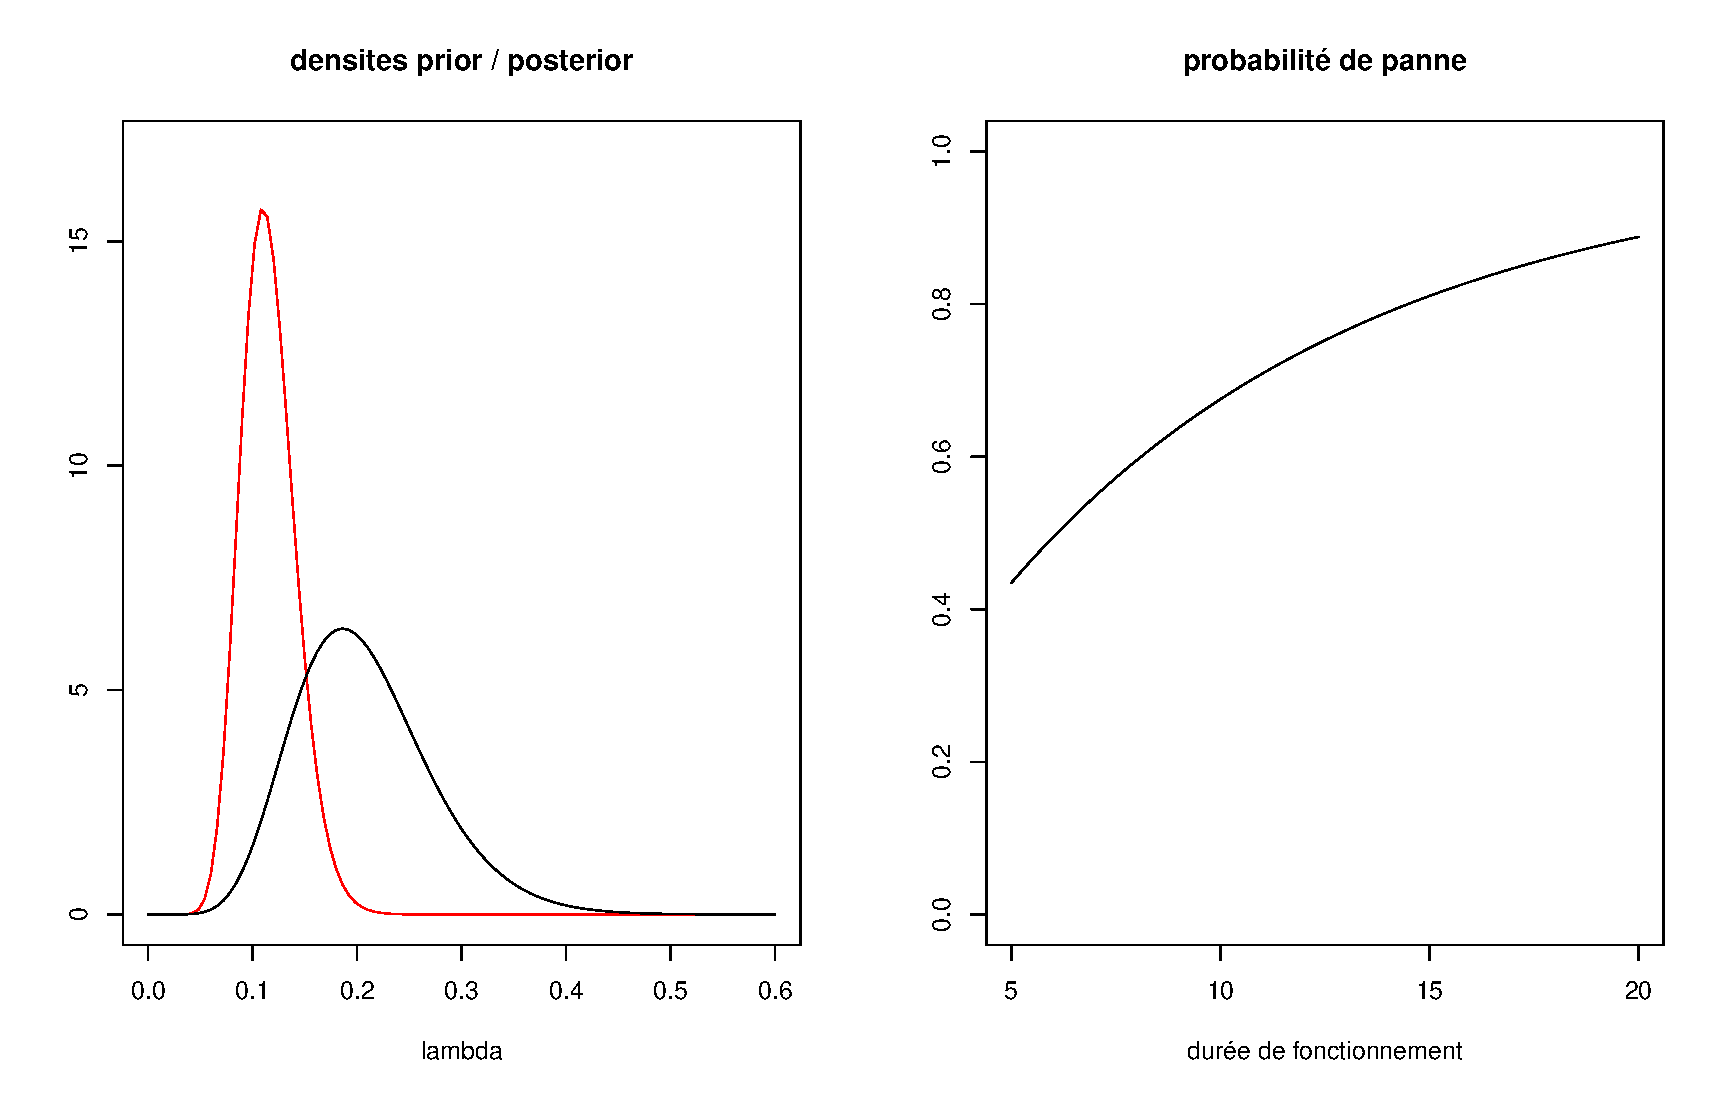
\includegraphics[scale=0.4]{figures/prior/figure02.pdf} 
\caption{$m=10$, $\bar{\lambda}=1/5$, $\alpha=50\%$ (expert très informatif et pessimiste).} \label{expert2}
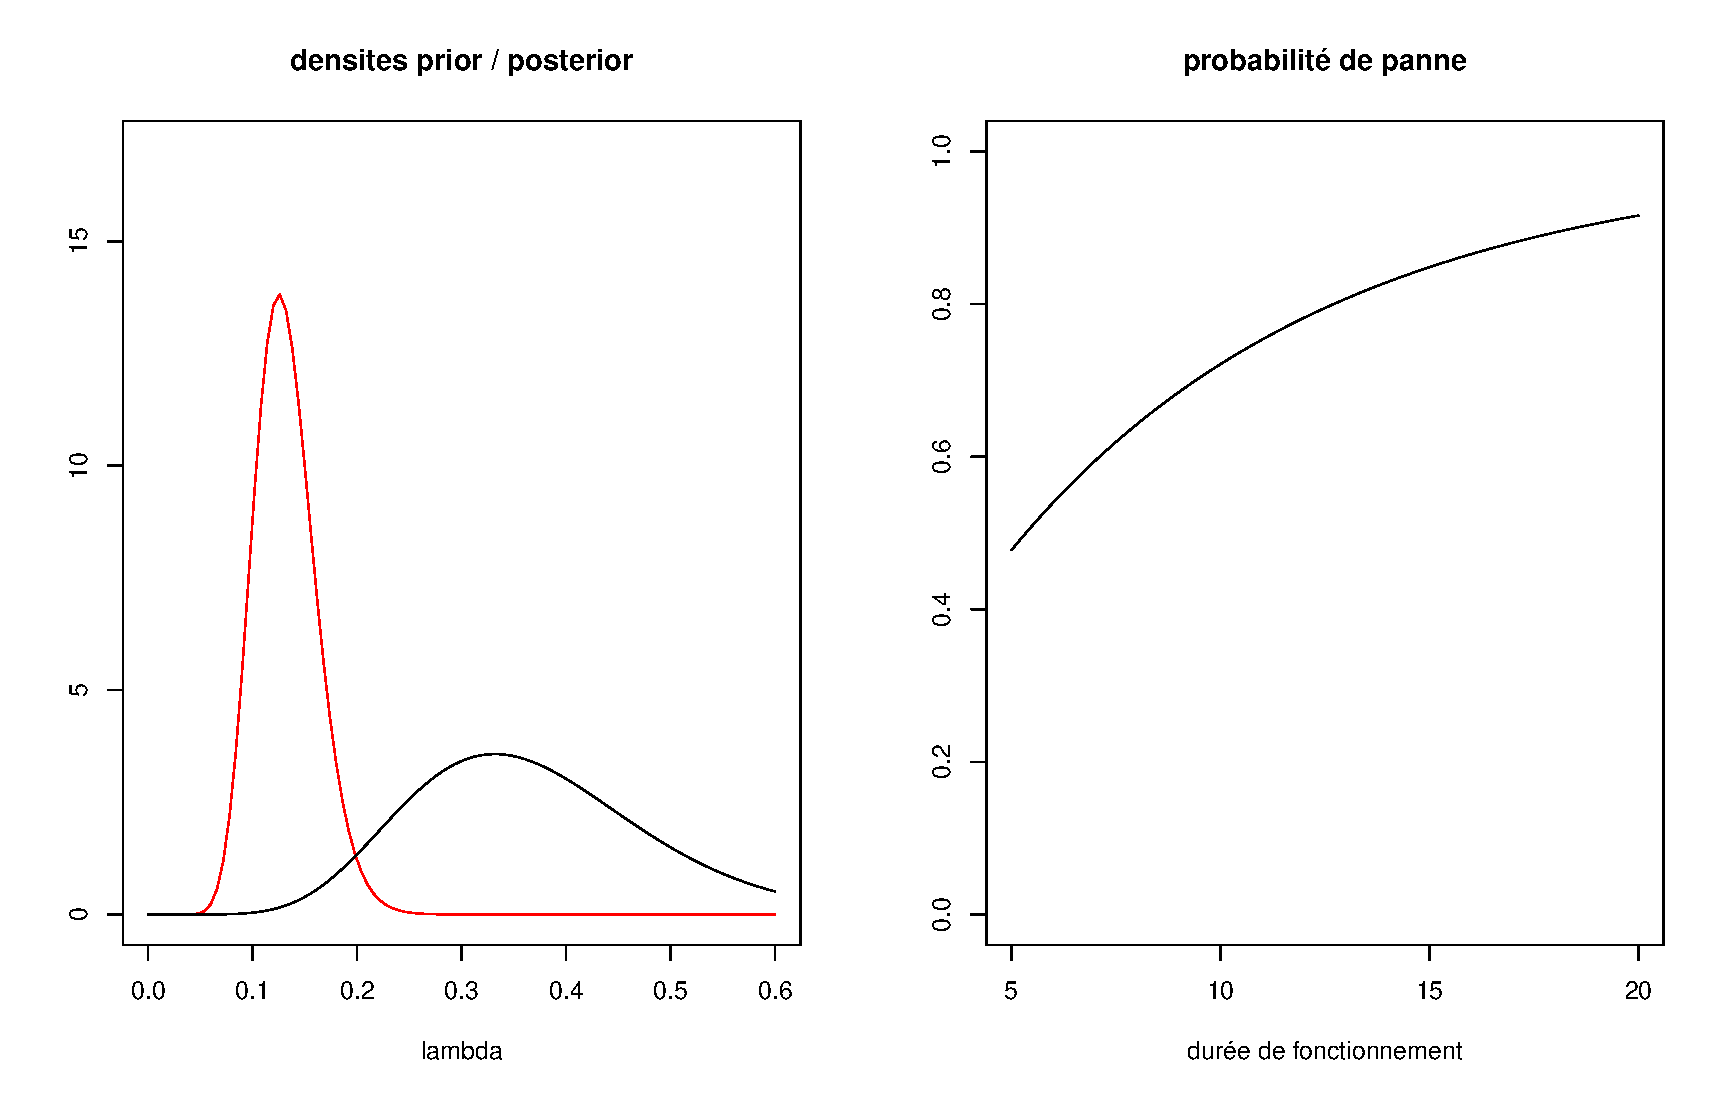
\includegraphics[scale=0.4]{figures/prior/figure03.pdf} 
\caption{$m=10$, $\bar{\lambda}=1/5$, $\alpha=5\%$ (expert très informatif et très pessimiste).} \label{expert3}
\end{figure}

En fait, plus habituellement, l'expert préfère exprimer son opinion \emph{quantitative} sur la durée de vie $X$
 ($=$ \emph{variable d'ancrage}) que sur $\lambda$, car $X$ est {\bf observable}. Dans ce cas, il est assimilé à un fournisseur d'estimé du \emph{quantile prédictif {\it a priori}} $\bar{x}$ :
\begin{eqnarray*}
\int_{0}^{\bar{x}} f(x) \ dx & = & \int_{0}^{\bar{x}} \int_{\Theta} f(x|\theta)\pi(\theta) \ d\theta \ = \ \alpha
\end{eqnarray*}
Cette interprétation est la plus acceptée en général dans la communauté statistique bayésienne, c'est pourquoi les statisticiens fiabilistes préfèrent poser des questions comme : 
\begin{eqnarray*}
\text{\it Sachant les temps $x_0$ et $x_1>x_0$, $\Sigma$ a $1-\alpha$ fois plus de chance de ne pas tomber en panne après $x_0$ qu'après $x_1$.} \\
\text{\it Quelle est votre évaluation de $1-\alpha$ ?} 
\end{eqnarray*}
%\item La réponse est un estimé de $\P(X>x_0)/P(X>x_1)$

\fi